\documentclass[11pt, a4paper]{article}
\usepackage{graphicx, fullpage, hyperref, listings}
\usepackage{appendix, pdfpages, color}
\usepackage{indentfirst} %段首空两格 棒
\usepackage{chngpage} 
\usepackage{tocloft}            % This squashes the Table of Contents a bit
\usepackage{pdfpages}
\usepackage{multirow}
\usepackage{amsmath}
\usepackage{framed}


\setlength\cftbeforesecskip{3pt}
\renewcommand{\contentsname}{\centerline{\textbf{Content}}}
\graphicspath{{images/}}

\usepackage{multicol}

\usepackage{graphicx}
\usepackage{epstopdf}
\hypersetup{CJKbookmarks,%
	bookmarksnumbered,%
	colorlinks,%
	linkcolor=black,%
	citecolor=black,%
	plainpages=false,%
	pdfstartview=FitH}

%%%%%%%代码语法高亮设置

\usepackage{color}

\definecolor{pblue}{rgb}{0.13,0.13,1}
\definecolor{pgreen}{rgb}{0,0.5,0}
\definecolor{pred}{rgb}{0.9,0,0}
\definecolor{pgrey}{rgb}{0.46,0.45,0.48}

\usepackage{listings}
\lstset{
	language=Java,
	showspaces=false,
	showtabs=false,
	%%%%%
	frame = single,
	stepnumber = 2,  
	numbersep = 4pt, 
	 numbers=left,
	%breakatwhitespace=false, 
	tabsize=2,  
	%%%%%
	breaklines=true,
	showstringspaces=false,
    breakatwhitespace=false, 
	commentstyle=\color{pgreen},
	keywordstyle=\color{pblue},
	stringstyle=\color{pred},
	basicstyle=\ttfamily,
	%moredelim=[il][\textcolor{pgrey}]{$$},
	%moredelim=[is][\textcolor{pgrey}]{\%\%}{\%\%},
}


%%%%%%%%代码语法高亮设置

\definecolor{MyLightYellow}{cmyk}{0,0.,0.2,0} 

\setlength{\parskip}{4pt}        % sets spacing between paragraphs
\interfootnotelinepenalty=500    % this prevents footnotes breaking across pages

\title{\includegraphics[width=0.45\textwidth]{wpi2}
        \\CS 534 Artificial Intelligence \\ Assignment 3 }          % <<<<<<<<< change the title as appropriate
\author{Group 10 }                    % <<<<<<<<< module code

\begin{document}
\begin{titlepage}
	
%\date{\today}
\maketitle
\addtocontents{toc}{\protect\thispagestyle{empty}} % because we don't want a page number on the title page
% Thanks to Huang Shanyue for suggesting this 

\begin{center}
Group Member
\end{center}

\begin{table}[htbp] 
\begin{center}
\begin{tabular}{l l l} 
	 
	 Yixuan & Jiao  &   yjiao@wpi.edu \\
     Yinkai & Ma  &   yma7@wpi.edu \\
     Jiaming & Nie  &  jnie@wpi.edu \\
     Pinyi & Xiao  &  pxiao@wpi.edu \\
\end{tabular}
\end{center}
\end{table}



%\date{\today}
\thispagestyle{empty}  %去除首页页码

\end{titlepage}

\section{Procedure of Expectation and Maximization}

The EM algorithm will initialize the related parameters $\theta$ as Gaussian distribution parameters, then perform the expectation and maximization process.


At the beginning, we randomly pick “K” number of points as the initial state, and then generate clusters by using reasonable variances. Then, we use “E-step” to calculate the probabilities of each point for being in the “K” different clusters, which is also known as the expected probability distribution. After having the probability distribution, we use “M-step” to recalculate the center points (mean) according to the probability distribution of “E-step” and find the new variance of each new cluster. Finally, repeat the “E-step” and “M-step” until the clusters convergent into stable clusters.

\subsection{Expectation Procedure}

\begin{itemize}
\item Calculate probability of data point $x_j$ belongs to cluster $i$ $P_{ij} = P(C=i|x_j)$
\item According to Bayes' theorem, $P_{ij} = \alpha P(x_j|C=i)P(C=i)$
\item $P(x_j|C=i)$ is the probability of point $x_j$ belongs to cluster $i$, $P(C=i)$ is the weight of the probability.
\item Calculate effective number $n_i = \sum P_{ij}$ of the data point is in cluster $i$.  
\end{itemize}

\subsection{Maximization Procedure}

In the Maximization procedure, the mean $\mu$ and variance ${\sigma}^2$ will be updated according to the result obtained in Expectation procedure.

\begin{equation}
	\mu_i = \sum P_{ij}/n_{i}
\end{equation}

\begin{equation}
	\sum_i = \sum_i P_{ij}(x_j - \mu_i){(x_j - \mu_i)}^{T}/n_i
\end{equation}

\begin{equation}
	w_i = n_i / N
\end{equation}

The expectation procedure is the process of calculation of expected value $P_{ij}$ with the hidden variable $Z_{ij}$. In the maximization procedure, the log-likelihood will be updated and the parameters of different Gaussian models.

\section{Random Starts and Number Determination}
\label{sec:2}
\subsection{Cluster Number Determination}

In the Extended EM part, the Bayesian Interference Criteria combined with the log-likelihood will be used to assess the clustering accuracy.

The log-likelihood is defined as the following:

\begin{equation}
	L(\theta) = \sum_i P(X_i,C_j|\theta_j)
\end{equation}

The equation of BIC is defined on the following:

\begin{equation}
BIC(k) = -2\times log_likelihood + k\times ln(N)
\end{equation}

In the iterations of log-likelihood, for different iterations, the log-likelihood and BIC values will vary to a large extent sometimes, which means that variance of the BIC will be large. The phenomenon will show up under some occasions that the cluster number is not very accurate. 

In this assignment, the variance $Var$ is given and the program will restart if the change exceeds some degree.

The calculation procedure is on the following:

\begin{itemize}
\item For certain cluster number $K$, calculate BIC
\item Random restart for cluster number $K$, obtain the result array of the BIC 
\item Calculate the variance $var$ of the BIC list, which will is used to assess the algorithm accuracy
\end{itemize}

\subsection{Restart Criteria}

The restart for certain cluster number $K$ will be performed for certain numbers.




\section{Initialization of Cluster Centers}

Given the cluster number $K$, random choose $K$ points from the data array as the cluster number.

We randomly pick $K$ number of points from the raw data as the initial cluster centers, and then initialize the clusters according to these centers. When this project initializes the variance of the center, the variance is randomly getting between the 1 times total data variance and 3 times total data variance. Such as, when $K=3$,  given a set of points, this project picks 3 different points of the data as the 3 clusters center. And then, calculate the variance of all the data, and get the variance of x and y, which is a, b, and then, set the variance of the cluster is random from a to 3a, b to 3b.

\section{Termination Criteria on EM Algorithm}

After each M-step, we have generated new centers of K clusters, then we compute the distance between the former center locations and the current center locations.

By adding up these distances together and dividing the sum with number “K”, we calculate a result measuring the progress of iteration. If the sum is larger than 0.1, then the iterations continue; if not, process complete and terminate it.

\section{Data File Generation}
\label{sec:5}

\subsection{Generated Data Description}

The data that we created includes 3 Gaussian distribution, the means of them are [0,0], [10,10] and [20,20], the variance of them are [[100,1], [1,100]], [[10,1], [1,10]] and [[50,1], [1,50]].
When using extended EM, the result is like that:

\subsection{Performance of EM Algorithm}

According to the part~\ref{sec:2}, the criteria is the variance of the random restart process of the calculation of BIC value.

The figure on the following:

\begin{figure}[htbp]
	
	\centering 
	\includegraphics[width=12cm]{5_2}
	
	\caption{Generated Data File}
	\label{fig:5-2}
	
\end{figure}

Through the calculation of the variance of the normalized BIC value, when cluster number $K=3$ gives the second best performance which is near to the $K=2$ clustering result. Other clustering results give the 2 or 3 orders of magnitude.


\subsection{Results o f the Extended EM Algorithm}

If given the correct number of the clusters, in this project, I give the k=3, and run the basic EM, could get the figure of the log-likelihood vs iteration is like the figure below~\ref{fig:5-3}:


\begin{figure}[htbp]
	
	\centering 
	\includegraphics[width=12cm]{5_3_1}
	
	\caption{Log-Likelihood vs. Iteration}
	\label{fig:5-3}
	
\end{figure}

\newpage

And get the means of three clusters are $\begin{bmatrix}
	10.160927305532486 & 10.311809083724215 \\ 0.3022128376500947 & -0.028573619938553493 \end{bmatrix}$, $ \begin{bmatrix}
10.160927305532486 & 10.311809083724215 \\ 0.3022128376500947 & -0.028573619938553493
	\end{bmatrix}$, $\begin{bmatrix}
		10.160927305532486 & 10.311809083724215 \\ 0.3022128376500947 & -0.028573619938553493 
	\end{bmatrix}$ and  [20.672087754598735, 19.641971376001067], and the variance of them are [[12.577488828945143, 0.5694856082850692], [-0.05267943518194221, 10.673271231583815]], [[100.80295507545482, -1.0269924937393347], [-6.828986119723152, 96.44827857518334]] and , [[45.8920741435162, 1.505551578403153], [2.8330470399896046, 42.72457103704982]], the result is close to the correct, so it could find the correct means and variances of the clusters. And it does not assign points to the correct cluster, it just give the probabilities of each point assign each cluster.




\section{Log-likelihood vs. Iterations}

In this section, the data file is the file generated in part~\ref{sec:5}. This data file has 3 clusters generated from 3 different Gaussian Distribution models.

In figure illustrated the plot of the data, the data is illustrated on the following:

\begin{figure}[htbp]
	
	\centering 
	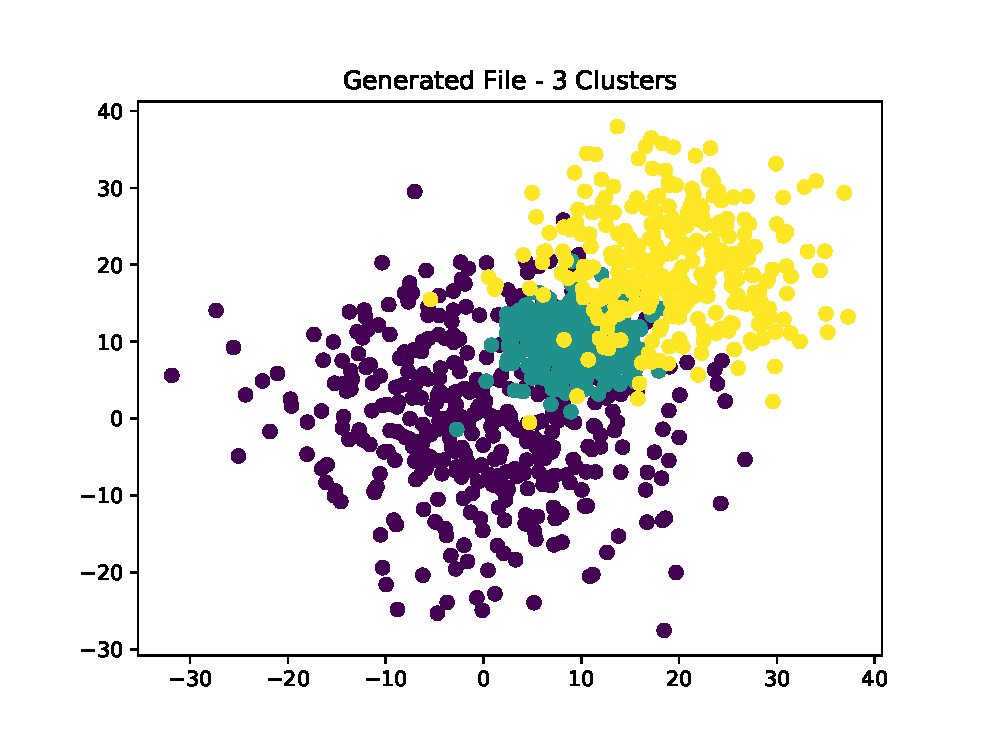
\includegraphics[width=12cm]{6.eps}
	
	\caption{Generated Data File}
	\label{fig:kf8}
	
\end{figure}

\newpage

\subsection{K=2 Log-Likelihood vs. Iteration}

For the cluster number $K=2$, the graph of the log-likelihood and iteration is illustrated in figure~\ref{fig:kf9}.

\begin{figure}[htbp]
	
	\centering 
	\includegraphics[width=8cm]{6_2.eps}
	
	\caption{K=2 Log-Likelihood vs. Iteration}
	\label{fig:kf9}
	
\end{figure}

\subsection{K=3 Log-Likelihood vs. Iteration}

For the cluster number $K=3$, the graph of the log-likelihood and iteration is illustrated in figure~\ref{fig:kf10}.

\begin{figure}[htbp]
	
	\centering 
	\includegraphics[width=6cm]{6_3.eps}
	
	\caption{K=3 Log-Likelihood vs. Iteration}
	\label{fig:kf10}
	
\end{figure}

\subsection{K=4 Log-Likelihood vs. Iteration}

For the cluster number $K=4$, the graph of the log-likelihood and iteration is illustrated in figure~\ref{fig:kf11}.

\begin{figure}[htbp]
	
	\centering 
	\includegraphics[width=8cm]{6_4.eps}
	
	\caption{K=4 Log-Likelihood vs. Iteration}
	\label{fig:kf11}
	
\end{figure}

\subsection{K=5 Log-Likelihood vs. Iteration}

For the cluster number $K=5$, the graph of the log-likelihood and iteration is illustrated in figure~\ref{fig:kf12}.

\begin{figure}[htbp]
	
	\centering 
	\includegraphics[width=6cm]{6_5.eps}
	
	\caption{K=5 Log-Likelihood vs. Iteration}
	\label{fig:kf12}
	
\end{figure}

\newpage

\subsection{K=6 Log-Likelihood vs. Iteration}

For the cluster number $K=6$, the graph of the log-likelihood and iteration is illustrated in figure~\ref{fig:kf13}.

\begin{figure}[htbp]
	
	\centering 
	\includegraphics[width=8cm]{6_6.eps}
	
	\caption{K=6 Log-Likelihood vs. Iteration}
	\label{fig:kf13}
	
\end{figure}

\subsection{K=7 Log-Likelihood vs. Iteration}

For the cluster number $K=7$, the graph of the log-likelihood and iteration is illustrated in figure~\ref{fig:kf14}.

\begin{figure}[htbp]
	
	\centering 
	\includegraphics[width=8cm]{6_7.eps}
	
	\caption{K=7 Log-Likelihood vs. Iteration}
	\label{fig:kf14}
	
\end{figure}


\newpage
\section{BIC Criteria and its Application}

The equation of the Bayesian Interference Criteria is on the following:

\begin{equation}
BIC(k) = -2\times log_likelihood + k\times ln(N)
\label{eq:bic}
\end{equation}

In the equation~\ref*{eq:bic}, $k$ is the number of the cluster, $N$ is the number of all the points.


In the part 2, the extended EM part, for one test file, assume there are several kinds of cluster $K$, for each hypothesis $K_i$, the EM algorithm will test 20 iterations for the estimation of log-likelihood and BIC.

The variance of the 20 iterations of each cluster $K_i$ will be a criteria to assess the stability of the accuracy of the clustering.

The cluster number $K_i$ which is near to the data original clustering will have the smallest variance.   

%\tableofcontents
%\listoffigures



%\tableofcontents

%\listoffigures
%\listoftables
%\lstlistoflistings        


%\newpage




\bibliographystyle{IEEEtran}  
%\bibliography{MyRefs} 
%\addcontentsline{toc}{section}{References}





%-------------------------------------------------------------------------------------------------------





\end{document}
